\chapter{Arhitektura i dizajn sustava}
		
	
	Arhitektura ovog projekta se može razlučiti na tri podsustava:
	\begin{packed_item}
	\setlength\itemindent{24pt}
		\item\textbf{Web aplikacija}
		\item\textbf{Web poslužitelj}
		\item\textbf{Baza podataka}
	\end{packed_item}
	
	\textbf{Web poslužitelj} je podsustav kojemu je zadaća spremanje, obrađivanje i dostavljanje klijentima sadržaj web stranica. Preko web aplikacije poslužitelj komunicira sa klijentom koji je u ovom slučaju web preglednik. Komunikacija se odvija putem protokola aplikacijskog sloja interneta - HTTP (Hypertext Transfer Protocol). On je tu da "reagira" na akcije koje mu web preglednik proslijedi te o ovisno o potrebi proljeđuje zahtjev na web aplikaciju.\\
	
	\textbf{Web preglednik} je program koji fizičkom korisniku omogućuje učitavanje i pregled web aplikacije. On je tu kao prevoditelj što znači da interpretira prikaz koda pisanog i uređivanog u HTML-u u izgled razumljiv
korisnicima. Putem web preglednika korisnik šalje HTTP zahtjeve web poslužitelju, no isto tako web poslužitelj je tu da prilagodi prikaz HTTP odgovora i prikaže ih korisniku.\\

	\textbf{Baza podataka} je podsustav u podatkovnom sloju kojem je primaran uloga sigurno spremanje podataka, a detaljnije o njoj se govori u poglavlju 4.1.\\
	
	\textbf{Web aplikacija} je dio sustava kojeg korisnik koristi za obrađivanje željenih zahtijeva koji uzrokuju pristupanje podacima u bazi podataka. Web aplikacija za interpretiranje dostavlja web pregledniku određeni HTML kod, a podijeljena je na back-end i na front-end o kojima je riječ u nastavku.
	\begin{packed_item}
	\item\textbf{Front-end} ili klijentska strana je dio aplikacije koji služi za sve ono vidljivo na web pregledniku. On je prezentacijski sloj koji korisniku omogućuje jednostavnu komunikaciju sa sustavom. Tehnologija koja je korištena za realizaciju ovog dijela web aplikacije je programski jezik JavaScript, preciznije radni okvir React u kombinaciji sa TypeScriptom.
	\item\textbf{Back-end} ili poslužiteljska stran je dio aplikacije koji je zadužan za obrađivanje dobivenih zahtjeva i vršenja funkcionalnih akcija. Tehnologija u kojom je pisan je programski jezik Java, preciznije u radnom okviru SpringBoot.\\
	\end{packed_item}

	Okruženje u kojem je pisan front-end je Visual Studio Code, a backe-end u Intellij-u. To nisu fiksna okruženja i može se koristiti bilo koji drugi IDE ili text editor. Arhitektura sustava se temelji na višeslojnom arhitekturnom stilu koji je podržan od strane SpringBoot tehnologije.\\
	
	\textbf{\underline{Višeslojni stil arhitekture}}\\
	Višeslojna arhitektura sastoji se od idućih slojeva:
	\begin{packed_item}
	\setlength\itemindent{24pt}
	\item klijentske strane koja omogućuje prikaz korisničkog sučelja
	\item nadglednika koji korisničku i poslužiteljsku stranu
	\item usluge koja obavlja poslovnu logiku i ostvaruje temeljnu funkcionalnost i zadaaću web aplikacije
	 \item repozitorija koji definira način pristupanja podacima
	 \item baze podataka koja u našem slučaju podatke sprema u relacijsku bazu Postgre\\
	\end{packed_item}
	
	Osnovna značajka ovakvog stila arhitekture su da svaki sloj pruža uslugu drugom sloju, a skriva svoj skup usluga. Jedna od prednosti ovog stila je olakšavanje ostvarivanja podjele brige u web aplikaciji jer se svaki sloj brine isključivo o svojoj funkcionalnosti. Klijentska strana razgovara sa web sučeljem, nadglednik putem REST API-ja pruža vanjsko sučelje i prihvaća HTTP zahtjeve te poziva odgovarajuće usluge, a potom te iste vraća kao odgovor klijentu. Sloj usluge definira pristup uslugama web aplikacije(tko i kako pristupa). Sloj repozitorija nam osigurava pristup podacima, te preslikavanje domenskih objekata u bazu podataka koristeći formu 1:1. Skica ovakve arhitekure je dana na slici \ref{fig:arhitektura}\\
	
	\begin{figure}[H]
			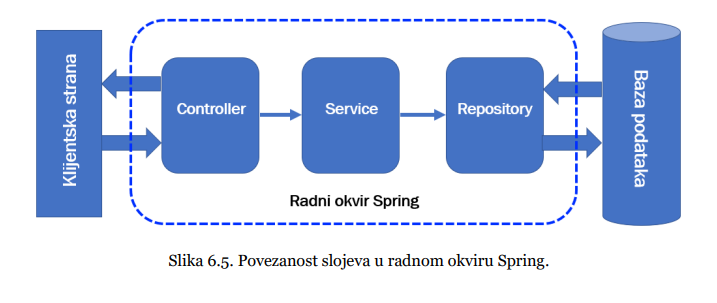
\includegraphics[scale=0.8]{slike/viseslojna_arhitekt.PNG} %veličina slike u odnosu na originalnu datoteku i pozicija slike
			\centering
			\caption{Primjer višeslojne arhitekture korištenjem radnog okvira Spring}
			\label{fig:arhitektura}
		\end{figure}

	
		

		

				
		\section{Baza podataka}
			
			\textbf{\textit{dio 1. revizije}}\\
			
		Za potrebe sustava koristit će se relacijska baza podataka koja nam omogućuje jednostavnije modeliranje stvarnog svijeta. Baza je implementirana u PostgreSQL-u zbog njegove jednostavnosti i jer je tim najbolje upoznat s tim sustavom; njegovim limitacijama i pravilima. Entiteti stvarnog svijeta su prevedeni kao tablice (relacije) koje imaju ime i svoj skup atributa. Baza podataka osigurava nam jednostavnu pohranu, umetanje, izmjenu i dohvat podataka, te garantira njihovu sigurnost. Baza podataka koristi sljedeće atribute:
		\begin{packed_item}
		\setlength\itemindent{24pt}
		\item Prijave
		\item Lokacije
		\item Slike
		\item Korisnici
		\item tipOstecenja
		\item Vijeca
		\end{packed_item}
		
		
			\subsection{Opis tablica}
			

				\textbf{Prijave} je entitet koji sadrži sve važne informacije o podnesenim prijavama. Sastoji se od atributa:id, ostecenjaId, lokacijaId, kreatorId, parentId, vrijemePrijave i vrijemeOtklona. Ovaj entitet u vezi je One-to-One s tablicom lokacije preko atributa lokacijaId, sa entitetom slike je u vezi One-to-Many preko atributa id. Sa entitetom tipOstecenja je u vezi One-to-Many preko atributa ostecenjeID, te je u vezi Many-to-One sa entitetom Korisnici preko atributa kreatorID.\\
				
				
				\begin{longtblr}[
					label=none,
					entry=none
					]{
						width = \textwidth,
						colspec={|X[6,l]|X[6, l]|X[20, l]|}, 
						rowhead = 1,
					} %definicija širine tablice, širine stupaca, poravnanje i broja redaka naslova tablice
					\hline \SetCell[c=3]{c}{\textbf{Prijave}}	 \\ \hline[3pt]
					\SetCell{LightGreen}id & INT & jedinstveni identifikator prijave  	\\ \hline
					\SetCell{LightBlue}ostecenjeId	& INT & jedinstveni identifikator tipa ostecenja   	\\ \hline 
					\SetCell{LightBlue}kreatorId & INT &  jedinstvani identifikator korisnika koji je poslao prijavu \\ \hline 
					\SetCell{LightBlue}parentId & INT & jedinstveni identifikator prijave na koju se prijava nadovezala		\\ \hline 
					 vrijemePrijave	& INT &  vrijeme slanja prijave 	\\ \hline
					 vrijemeOtklona	& INT &  vrijeme otklona prijave 	\\ \hline 
					\end{longtblr}
					
					\textbf{Lokacije} je entitet koji sadrži osnovne podatke o geografskoj lokaciji pojedine prijave. Sastoji se od atributa: id, latitude, longitude. Preko atributa id je povezana vezom One-to-One sa relacijom Prijave.\\
				
				\begin{longtblr}[
					label=none,
					entry=none
					]{
						width = \textwidth,
						colspec={|X[6,l]|X[6, l]|X[20, l]|}, 
						rowhead = 1,
					} %definicija širine tablice, širine stupaca, poravnanje i broja redaka naslova tablice
					\hline \SetCell[c=3]{c}{\textbf{Lokacije}}	 \\ \hline[3pt]
					\SetCell{LightGreen}id & INT &  	jedinstveni identifikator prijave 	\\ \hline
					latitude & INT & geografska latituda lokacije   	\\ \hline 
					longitude & INT & geografska longituda lokacije   	\\ \hline 
				\end{longtblr}
				
				\textbf{Korisnici} je entitet koji sadrži osobne podatke o registriranim korisnicima kao i njihovu pripadnost vijecu i ulogu koju obnašaju u sustavu. Sastoji se od atributa: id, ime, prezime, username, email, passwordHash, vijeceId, token, role. Povezani su sa relacijom Prijave u vezi One-to-Many preko atributa id, te sa relacijom Vijeca u vezi Many-to-One preko atributa vijeceId.\\
				
				\begin{longtblr}[
					label=none,
					entry=none
					]{
						width = \textwidth,
						colspec={|X[6,l]|X[6, l]|X[20, l]|}, 
						rowhead = 1,
					} %definicija širine tablice, širine stupaca, poravnanje i broja redaka naslova tablice
					\hline \SetCell[c=3]{c}{\textbf{Korisnici}}	 \\ \hline[3pt]
					\SetCell{LightGreen}id & INT & jedinstveni identifikator korisnika  	\\ \hline
					ime	& VARCHAR & ime registriranog korisnika   	\\ \hline
					prezime	& VARCHAR & prezime registriranog korisnika   	\\ \hline
					username	& VARCHAR & korisničko ime registriranog korisnika   	\\ \hline 
					email & VARCHAR & e-mail adresa registriranog korisnika   	\\ \hline
					passwordHash	& VARCHAR & lozinka za prijavu registriranog korisnika   	\\ \hline
					\SetCell{LightBlue}vijeceId & INT &  jedinstvani identifikator vijeca/ureda kojem pripada \\ \hline 
					token & INT & jedinstveni identifikator prijave na koju se prijava nadovezala		\\ \hline 
					 role & VARCHAR &  uloga koju korisnik obnaša u sustavu 	\\ \hline 
				\end{longtblr}
				
				\textbf{Slike} je entitet koji sadrži podatke vezane za sliku podnešene prijave. Sastoji se od atributa: id, podatak, prijavaId. Preko entiteta prijavaId je povezan tablicom Prijave u vezi Many-to-One.\\
				
				\begin{longtblr}[
					label=none,
					entry=none
					]{
						width = \textwidth,
						colspec={|X[6,l]|X[6, l]|X[20, l]|}, 
						rowhead = 1,
					} %definicija širine tablice, širine stupaca, poravnanje i broja redaka naslova tablice
					\hline \SetCell[c=3]{c}{\textbf{slike}}	 \\ \hline[3pt]
					\SetCell{LightGreen}id & INT &  	jedinstveni identifikator slike pojedine prijave	\\ \hline
					podatak & VARCHAR & geografska latituda lokacije   	\\ \hline 
					\SetCell{LightBlue}prijavaId & INT & jedinstveni identifikator prijave za koju je poslana slika   	\\ \hline 
				\end{longtblr}
				
				\textbf{tipOstecenja} je entitet koji sadrži podatke vezane za opis oštećenja kao i id ureda koji se bavi tim tipom oštećenja. Sastoji se od atributa: id, naziv, vijeceId. Preko atributa id je povezan sa relacijom Prijave u vezi Many-to-One, te je sa relacijom Vijeca u vezi One-to-One povezan preko atributa vijeceId\\
				
				\begin{longtblr}[
					label=none,
					entry=none
					]{
						width = \textwidth,
						colspec={|X[6,l]|X[6, l]|X[20, l]|}, 
						rowhead = 1,
					} %definicija širine tablice, širine stupaca, poravnanje i broja redaka naslova tablice
					\hline \SetCell[c=3]{c}{\textbf{tipOstecenja}}	 \\ \hline[3pt]
					\SetCell{LightGreen}id & INT &  	jedinstveni identifikator vrste oštećenja	\\ \hline
					naziv & VARCHAR & naziv konkretnog oštećenja   	\\ \hline 
					\SetCell{LightBlue}vijeceId & INT & jedinstveni identifikator vijeca koji je zadužen za taj tip oštećenja   	\\ \hline 
				\end{longtblr}
				
				\textbf{Vijeca} je entitet koji sadrži podatke vezane za opis pojedinog vijeca/ureda koji je zadužen za otklanjanje određenog tipa oštećenja. Sastoji se od atributa: id i naziv. Preko atributa id je povezan sa relacijom tipOstecenja u vezi One-to-One, te je povezan sa relacijom Korisnici preko atributa id u vezi One-to-Many.\\
				
				\begin{longtblr}[
					label=none,
					entry=none
					]{
						width = \textwidth,
						colspec={|X[6,l]|X[6, l]|X[20, l]|}, 
						rowhead = 1,
					} %definicija širine tablice, širine stupaca, poravnanje i broja redaka naslova tablice
					\hline \SetCell[c=3]{c}{\textbf{Vijeca}}	 \\ \hline[3pt]
					\SetCell{LightGreen}id & INT &  jedinstveni identifikator pojedinog registriranog vijeća/ureda	\\ \hline
					naziv & VARCHAR & puni naziv vijćea u aplikaciji\\ \hline 
				\end{longtblr}
				
				
			
			\subsection{Dijagram baze podataka}
				\begin{figure}[H]
			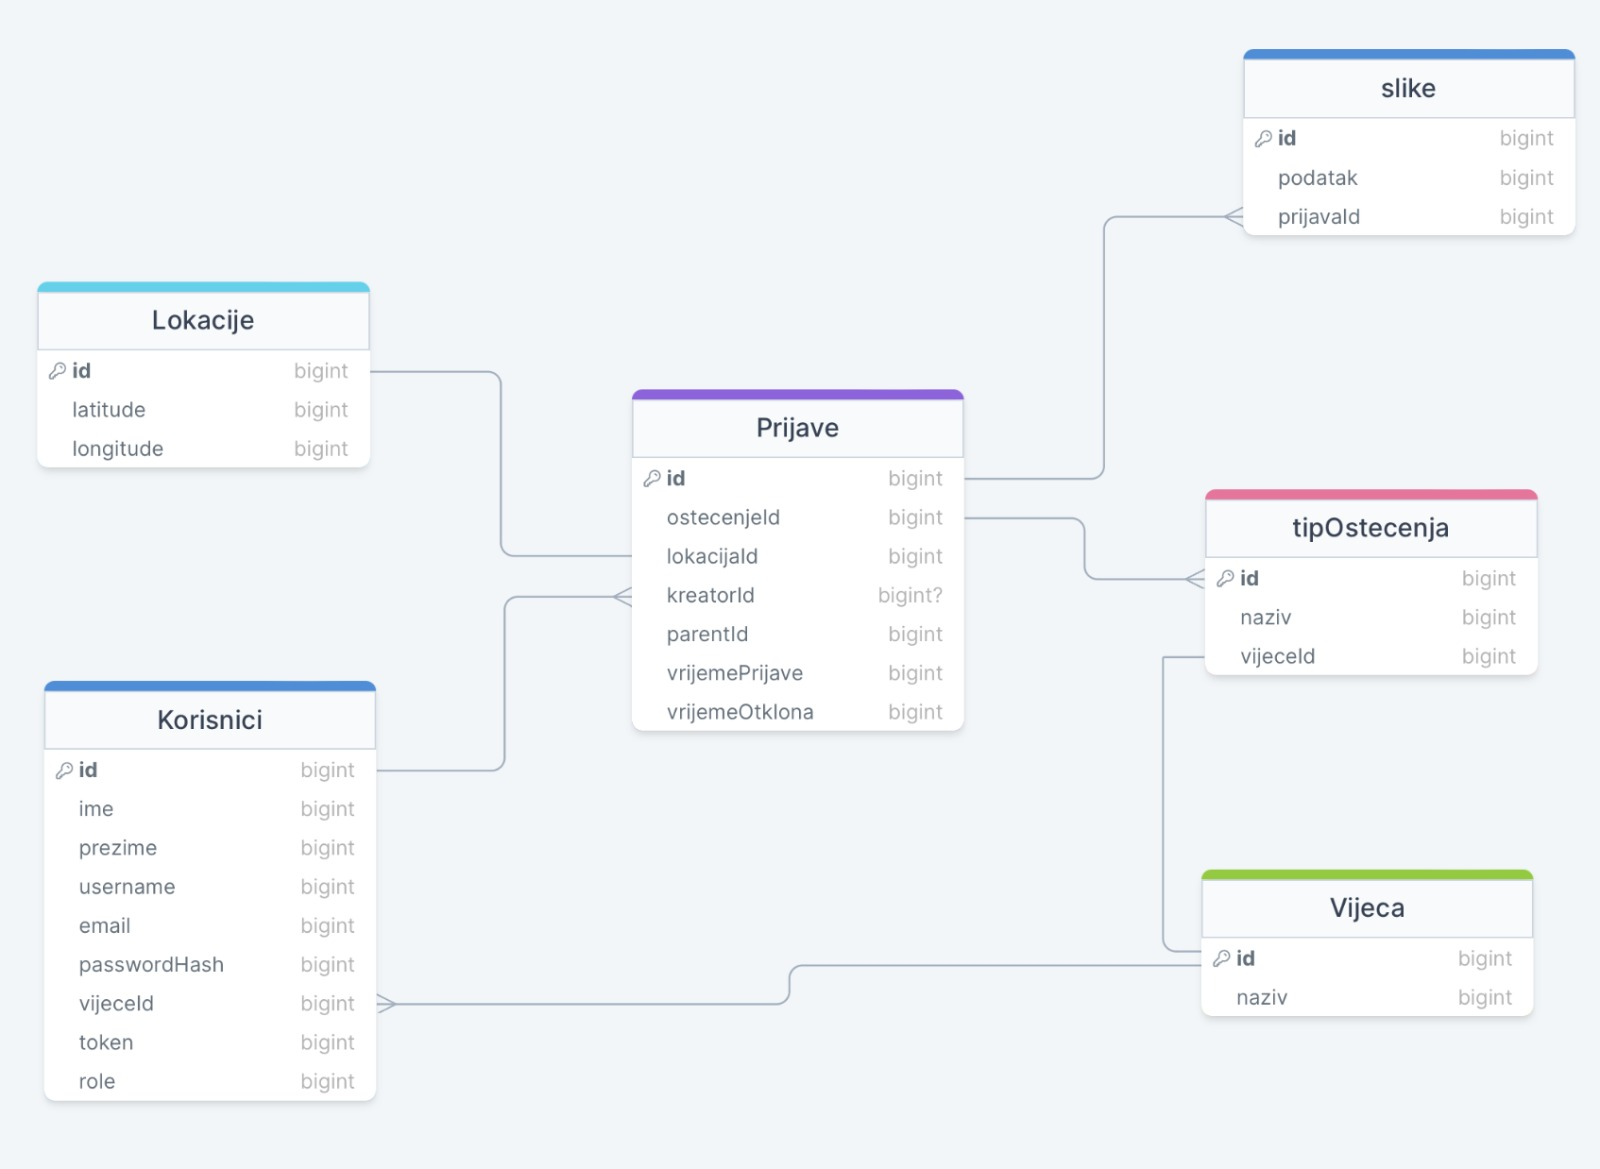
\includegraphics[scale=0.3]{slike/bazaPodataka.PNG} %veličina slike u odnosu na originalnu datoteku i pozicija slike
			\centering
			\caption{Relacijski dijagram baze podataka}
			\label{fig:bazapod}
		\end{figure}
			
			\eject
			
			
		\section{Dijagram razreda}
		
			\textit{Potrebno je priložiti dijagram razreda s pripadajućim opisom. Zbog preglednosti je moguće dijagram razlomiti na više njih, ali moraju biti grupirani prema sličnim razinama apstrakcije i srodnim funkcionalnostima.}\\
			
			\textbf{\textit{dio 1. revizije}}\\
			
			\textit{Prilikom prve predaje projekta, potrebno je priložiti potpuno razrađen dijagram razreda vezan uz \textbf{generičku funkcionalnost} sustava. Ostale funkcionalnosti trebaju biti idejno razrađene u dijagramu sa sljedećim komponentama: nazivi razreda, nazivi metoda i vrste pristupa metodama (npr. javni, zaštićeni), nazivi atributa razreda, veze i odnosi između razreda.}\\
			
			\textbf{\textit{dio 2. revizije}}\\			
			
			\textit{Prilikom druge predaje projekta dijagram razreda i opisi moraju odgovarati stvarnom stanju implementacije}
			
			
			
			\eject
		
		\section{Dijagram stanja}
			
			
			\textbf{\textit{dio 2. revizije}}\\
			
			\textit{Potrebno je priložiti dijagram stanja i opisati ga. Dovoljan je jedan dijagram stanja koji prikazuje \textbf{značajan dio funkcionalnosti} sustava. Na primjer, stanja korisničkog sučelja i tijek korištenja neke ključne funkcionalnosti jesu značajan dio sustava, a registracija i prijava nisu. }
			
			
			\eject 
		
		\section{Dijagram aktivnosti}
			
			\textbf{\textit{dio 2. revizije}}\\
			
			 \textit{Potrebno je priložiti dijagram aktivnosti s pripadajućim opisom. Dijagram aktivnosti treba prikazivati značajan dio sustava.}
			
			\eject
		\section{Dijagram komponenti}
		
			\textbf{\textit{dio 2. revizije}}\\
		
			 \textit{Potrebno je priložiti dijagram komponenti s pripadajućim opisom. Dijagram komponenti treba prikazivati strukturu cijele aplikacije.}